\section{Scanning motion}\label{ssec:scanning_motion}
In \cref{ssec:SPADs}, it was concluded that a SPAD array with one SPAD per pixel is not feasible. Therefore a scanning motion is required. Possible scanning motions for different SPAD array configurations are shown in \cref{tkz:scanning_motions}. Note that the $2048\times1$ motion is in essence a special case of the $2048\times N$ motion, where exactly one row of pixels is observed at a time. The $M\times N$, with $M<2048$ and $N<2048$ needs a scanning motion in both $x$ and $y$ direction. This makes the scanning motion very complicated and unreliable. Therefore only the family of solutions with $2048\times N$ with $N<2048$ will be considered.


\begin{figure}[H]
    \centering
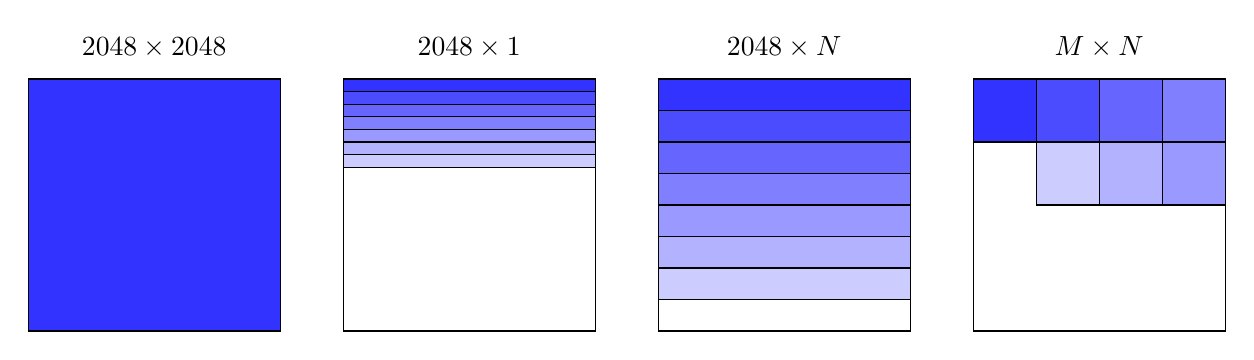
\begin{tikzpicture}[scale=.8]
\draw  (-3,4) rectangle (1,0);
\draw [fill=blue!80] (-3,4) rectangle (1,3.8);
\draw [fill=blue!70] (-3,3.8) rectangle (1,3.6);
\draw [fill=blue!60] (-3,3.6) rectangle (1,3.4);
\draw [fill=blue!50] (-3,3.4) rectangle (1,3.2);
\draw [fill=blue!40] (-3,3.2) rectangle (1,3);
\draw [fill=blue!30] (-3,3) rectangle (1,2.8);
\draw [fill=blue!20] (-3,2.8) rectangle (1,2.6);


\draw  (2,4) rectangle (6,0);
\draw [fill=blue!80] (2,4) rectangle (6,3.5);
\draw [fill=blue!70] (2,3.5) rectangle (6,3);
\draw [fill=blue!60] (2,3) rectangle (6,2.5);
\draw [fill=blue!50] (2,2.5) rectangle (6,2);
\draw [fill=blue!40] (2,2) rectangle (6,1.5);
\draw [fill=blue!30] (2,1.5) rectangle (6,1);
\draw [fill=blue!20] (2,1) rectangle (6,0.5);


\draw  (7,4) rectangle (11,0);
\draw [fill=blue!80] (7,4) rectangle (8,3);
\draw [fill=blue!70] (8,4) rectangle (9,3);
\draw [fill=blue!60] (9,4) rectangle (10,3);
\draw [fill=blue!50] (10,4) rectangle (11,3);
\draw [fill=blue!40] (10,3) rectangle (11,2);
\draw [fill=blue!30] (9,3) rectangle (10,2);
\draw [fill=blue!20] (8,3) rectangle (9,2);

\node at (-6,4.5) {$2048\times2048$};
\node at (-1,4.5) {$2048\times1$};
\node at (4,4.5) {$2048\times N$};
\node at (9,4.5) {$M\times N$};

\draw [fill=blue!80] (-8,4) rectangle (-4,0);
\end{tikzpicture}
    \caption{Different types of scanning motions}
    \label{tkz:scanning_motions}
\end{figure}
